%%%%%%%%%%%%%%%%%%%%%%%%%%%%%%%%%%%%%%%%%
% Lachaise Assignment
% LaTeX Template
% Version 1.0 (26/6/2018)
%
% This template originates from:
% http://www.LaTeXTemplates.com
%
% Authors:
% Marion Lachaise & François Févotte
% Vel (vel@LaTeXTemplates.com)
%
% License:
% CC BY-NC-SA 3.0 (http://creativecommons.org/licenses/by-nc-sa/3.0/)
% 
%%%%%%%%%%%%%%%%%%%%%%%%%%%%%%%%%%%%%%%%%

%----------------------------------------------------------------------------------------
%	PACKAGES AND OTHER DOCUMENT CONFIGURATIONS
%----------------------------------------------------------------------------------------

\documentclass{report}

%%%%%%%%%%%%%%%%%%%%%%%%%%%%%%%%%%%%%%%%%
% Lachaise Assignment
% Structure Specification File
% Version 1.0 (26/6/2018)
%
% This template originates from:
% http://www.LaTeXTemplates.com
%
% Authors:
% Marion Lachaise & François Févotte
% Vel (vel@LaTeXTemplates.com)
%
% License:
% CC BY-NC-SA 3.0 (http://creativecommons.org/licenses/by-nc-sa/3.0/)
% 
%%%%%%%%%%%%%%%%%%%%%%%%%%%%%%%%%%%%%%%%%

%----------------------------------------------------------------------------------------
%	PACKAGES AND OTHER DOCUMENT CONFIGURATIONS
%----------------------------------------------------------------------------------------

\usepackage{amsmath,amsfonts,stmaryrd,amssymb} % Math packages
\usepackage{enumerate} % Custom item numbers for enumerations
\usepackage{subfiles}
\usepackage{blindtext}
\usepackage{wrapfig}
\usepackage{multirow}
\usepackage{tabu}

\usepackage[utf8]{inputenc}
\usepackage{graphicx}
\usepackage{array}
\graphicspath{ {images/} }
\usepackage{float}
\usepackage{mathtools}
\DeclarePairedDelimiter\ceil{\lceil}{\rceil}
\DeclarePairedDelimiter\floor{\lfloor}{\rfloor}

\usepackage[ruled]{algorithm2e} % Algorithms
\usepackage[framemethod=tikz]{mdframed} % Allows defining custom boxed/framed environments
\usepackage{listings} % File listings, with syntax highlighting
\lstset{
	basicstyle=\ttfamily, % Typeset listings in monospace font
}

\RequirePackage[sfdefault]{ClearSans}
\RequirePackage[T1]{fontenc}
\RequirePackage{tikz}
\RequirePackage{xcolor}
\RequirePackage[absolute,overlay]{textpos}
\RequirePackage{ragged2e}
\RequirePackage{etoolbox}
\RequirePackage{ifmtarg}
\RequirePackage{ifthen}
\RequirePackage{pgffor}
\RequirePackage{marvosym}
\RequirePackage{parskip}

\DeclareOption*{\PassOptionsToClass{\CurrentOption}{article}}
\ProcessOptions\relax

%----------------------------------------------------------------------------------------
%	 SIDEBAR DEFINITIONS
%----------------------------------------------------------------------------------------

\setlength{\TPHorizModule}{1cm} % Left margin
\setlength{\TPVertModule}{1cm} % Top margin

\newlength\imagewidth
\newlength\imagescale
\pgfmathsetlength{\imagewidth}{5cm}
\pgfmathsetlength{\imagescale}{\imagewidth/600}

\newlength{\TotalSectionLength} % Define a new length to hold the remaining line width after the section title is printed
\newlength{\SectionTitleLength} % Define a new length to hold the width of the section title
\newcommand{\profilesection}[1]{%
	\setlength\TotalSectionLength{\linewidth}% Set the total line width
	\settowidth{\SectionTitleLength}{\huge #1 }% Calculate the width of the section title
	\addtolength\TotalSectionLength{-\SectionTitleLength}% Subtract the section title width from the total width
	\addtolength\TotalSectionLength{-2.22221pt}% Modifier to remove overfull box warning
	\vspace{8pt}% Whitespace before the section title
	{\color{black!80} \huge #1 \rule[0.15\baselineskip]{\TotalSectionLength}{1pt}}% Print the title and auto-width rule
}

% Define custom commands for CV info
\newcommand{\cvdate}[1]{\renewcommand{\cvdate}{#1}}
\newcommand{\cvmail}[1]{\renewcommand{\cvmail}{#1}}
\newcommand{\cvnumberphone}[1]{\renewcommand{\cvnumberphone}{#1}}
\newcommand{\cvaddress}[1]{\renewcommand{\cvaddress}{#1}}
\newcommand{\cvsite}[1]{\renewcommand{\cvsite}{#1}}
\newcommand{\aboutme}[1]{\renewcommand{\aboutme}{#1}}
\newcommand{\profilepic}[1]{\renewcommand{\profilepic}{#1}}
\newcommand{\cvname}[1]{\renewcommand{\cvname}{#1}}
\newcommand{\cvjobtitle}[1]{\renewcommand{\cvjobtitle}{#1}}

% Command for printing the contact information icons
\newcommand*\icon[1]{\tikz[baseline=(char.base)]{\node[shape=circle,draw,inner sep=1pt, fill=mainblue,mainblue,text=white] (char) {#1};}}

%----------------------------------------------------------------------------------------
%	 SIDEBAR LAYOUT
%----------------------------------------------------------------------------------------

\newcommand{\makeprofiles}{
	\begin{tikzpicture}[remember picture,overlay]
   		\node [rectangle, fill=sidecolor, anchor=north, minimum width=9cm, minimum height=\paperheight+1cm] (box) at (-5cm,3cm){};
	\end{tikzpicture}

	%------------------------------------------------

	\begin{textblock}{6}(0.5, 2)
			
		%------------------------------------------------
		
		\ifthenelse{\equal{\profilepic}{}}{}{
			\begin{center}
				\begin{tikzpicture}[x=\imagescale,y=-\imagescale]
					\clip (600/2, 567/2) circle (567/2);
					\node[anchor=north west, inner sep=0pt, outer sep=0pt] at (0,0) {\includegraphics[width=\imagewidth]{\profilepic}};
				\end{tikzpicture}
			\end{center}
		}

		%------------------------------------------------

		{\Huge\color{mainblue}\cvname}

		%------------------------------------------------

		{\Large\color{black!80}\cvjobtitle}

		%------------------------------------------------

		\renewcommand{\arraystretch}{1.6}
		\begin{tabular}{p{0.5cm} @{\hskip 0.5cm}p{5cm}}
			\ifthenelse{\equal{\cvdate}{}}{}{\textsc{\Large\icon{\Info}} & \cvdate\\}
			\ifthenelse{\equal{\cvaddress}{}}{}{\textsc{\Large\icon{\Info}} & \cvaddress\\}
			\ifthenelse{\equal{\cvnumberphone}{}}{}{\textsc{\Large\icon{\Info}} & \cvnumberphone\\}
			\ifthenelse{\equal{\cvsite}{}}{}{\textsc{\Large\icon{\Info}} & \cvsite\\}
			\ifthenelse{\equal{\cvmail}{}}{}{\textsc{\large\icon{\Info}} & \href{mailto:\cvmail}{\cvmail}}
		\end{tabular}

	
	\end{textblock}
}

%----------------------------------------------------------------------------------------
%	 COLOURS
%----------------------------------------------------------------------------------------

\definecolor{white}{RGB}{255,255,255}
\definecolor{gray}{HTML}{4D4D4D}
\definecolor{sidecolor}{HTML}{E7E7E7}
\definecolor{mainblue}{HTML}{0E5484}
\definecolor{maingray}{HTML}{B9B9B9}

%----------------------------------------------------------------------------------------
%	DOCUMENT MARGINS
%----------------------------------------------------------------------------------------

\usepackage{geometry} % Required for adjusting page dimensions and margins

\geometry{
	paper=a4paper, % Paper size, change to letterpaper for US letter size
	top=2.5cm, % Top margin
	bottom=3cm, % Bottom margin
	left=2cm, % Left margin
	right=2cm, % Right margin
	headheight=12pt, % Header height
	footskip=1.5cm, % Space from the bottom margin to the baseline of the footer
	headsep=0cm, % Space from the top margin to the baseline of the header
	%showframe, % Uncomment to show how the type block is set on the page
}

%----------------------------------------------------------------------------------------
%	 COLOURED SECTION TITLE BOX
%----------------------------------------------------------------------------------------

% Command to create the rounded boxes around the first three letters of section titles
\newcommand*\round[2]{%
	\tikz[baseline=(char.base)]\node[anchor=north west, draw,rectangle, rounded corners, inner sep=1.6pt, minimum size=5.5mm, text height=3.6mm, fill=#2,#2,text=white](char){#1};%
}

\newcounter{colorCounter}
\newcommand{\sectioncolor}[1]{%
	{%
		\round{#1}{
			\ifcase\value{colorCounter}%
			maingray\or%
			mainblue\or%
			maingray\or%
			mainblue\or%
			maingray\or%
			mainblue\or%
			maingray\or%
			mainblue\or%
 			maingray\or%
			mainblue\else%
			maingray\fi%
		}%
	}%
	\stepcounter{colorCounter}%
}

\newcommand{\parte}[1]{
	{%
		\color{gray}%
		\Large\sectioncolor{#1}%
	}
}

\newcommand{\subparte}[1]{
	\par\vspace{.5\parskip}{%
		\large\color{gray} #1%
	}
	\par\vspace{.25\parskip}%
}

%----------------------------------------------------------------------------------------
%	FONTS
%----------------------------------------------------------------------------------------

\usepackage[utf8]{inputenc} % Required for inputting international characters
\usepackage[T1]{fontenc} % Output font encoding for international characters
\usepackage{XCharter} % Use the XCharter fonts

%%%%%%%%%%%%%%%%%%%%%%%%%%%%%%%%%%%%%%%%%%%%%%%%%%%%%%%

\newenvironment{changemargin}[2]{%
\begin{list}{}{%
\setlength{\topsep}{0pt}%
\setlength{\topmargin}{#1}%
\setlength{\leftmargin}{#2}%
\setlength{\listparindent}{\parindent}%
\setlength{\itemindent}{\parindent}%
\setlength{\parsep}{\parskip}%
}%
\item[]}{\end{list}}
\RequirePackage{hyperref}
 % Include the file specifying the document structure and custom commands

%----------------------------------------------------------------------------------------
%	ASSIGNMENT INFORMATION
%----------------------------------------------------------------------------------------

\title{\vspace{-2cm}CALCULATOR: The Champernowne Constant (C10)} % Title of the assignment

\author{Nellybett Irahola\\ \texttt{ID \#40079991}\\ \texttt{Repository:https://github.com/NellybettIrahola/SOEN6481-Calculator}} % Author name and email address

\date{Concordia University--- August 02, 2019} % University, school and/or department name(s) and a date

%----------------------------------------------------------------------------------------

\begin{document}

\maketitle % Print the title
\listoffigures
\listoftables
\tableofcontents{}
%%%%%%%%%%%%%%%%%%%%%%%%%%%%%%%
\chapter{Introduction}

This project is based in the development of a calculator that computes the value of the Champernowne Constant (C10) and perform several operations that reflect its different uses. 

The purpose of the project is to engage with all the different concepts involved in the Requirement Specification Process. The calculator follows the user interests and expected functionalities.

In this project the first problem will present the user stories. The second problem will present a backwards traceability matrix and the last one will show the details of the implementation of the calculator.

\newpage
%----------------------------------------------------------------------------------------
%	BODY
%----------------------------------------------------------------------------------------
\chapter{Problems}

\section{PROBLEM 6: User Stories}

\subsection{Description}

The user stories' information will be presented in two sections. The first one with a table containing the id, description, priority, frequency of use, category and estimation. The estimation point of reference is one day which is represented by 8. The scale is defined using the fibonacci numbers.

The range for the priority and frequency is like the one provided by the CalCentral project [1]. It uses three levels Low, Medium and High.

The second section will present the constraints, acceptance test and acceptance criteria for the user stories. The constraints are presented by the relation with a non-functional requirement such as usability, flexibility, efficiency, security and others.

\subsection{User Stories Characteristics}

\begin{table}[H]
\centering
\begin{tabular}{ | m{2.7em} | m{8cm}| m{1.8cm} | m{1.5cm} | m{1.5cm} | m{1.5cm} |} 
\hline
ID & User Story Description & Category & Priority & Frequency & Estimation (Story points) \\ 
\hline
EN-US-1 & A student can use the calculator to show the decimal expansion of the Champernowne Constant in different bases, so he can get a better understanding of its behaviour for their research. & Research \& Learning & High & High & 5\\ 
\hline
EN-US-2 & A Number's Theory specialist can use the calculator to verify the presence of a numeric pattern in the Champernowne Constant, so they can confirm the characteristics of normal numbers and use it for their research. & Research & Medium & Low & 3 \\ 
\hline
EN-US-3 & A student can use the calculator to encrypt messages using a substitution cipher based on the number, so they can use it for their projects. & Learning \& Security & High & High & 5 \\ 
\hline
EN-US-4 & A student can use the calculator to decrypt messages using a substitution cipher based on the number and a key, so they can use it for their projects. & Learning \& Security & High & High & 5 \\ 
\hline
EN-US-5 & A student can use the calculator to encrypt messages using a one-time pad cipher based on the number, so they can use it for their projects. & Learning \& Security & High & High & 8 \\ 
\hline
EN-US-6 & A student can use the calculator to decrypt messages using a one-time pad cipher based on the number, so they can use it for their projects. & Learning \& Security & High & High & 8 \\ 
\hline
EN-US-7 & A student can use the calculator to perform elementary arithmetic operations that involve the number, so he can use it for specific calculations in his work. & Learning \& Research & Medium & High & 8 \\ 
\hline
EN-US-8 & A Number's Theory specialist can use the calculator to show the continued fraction expansion of the Champernowne Constant, so they evaluate some characteristics of the number and use it for their research. & Learning \& Research & Low & Low & 2 \\ 
\hline
EN-US-9 & A software engineer can use the calculator to show random numbers generated base on the Champernowne Constant, so they can use it for some interface features in their systems. & Learning \& Work & Low & Low & 3 \\ 
\hline
EN-US-10 & A student can use the calculator to show a graph of the number, so they can study their behaviour for their research. & Learning \& Research & Medium & Low & 5 \\ 
\hline
 
\hline
\end{tabular}
\caption[User Stories]{User Stories. Personal Creation.}
\label{table:1}
\end{table}


\subsection{Global Constraints} 

\textbf{Usability:} The program doesn't provide the option of increasing the size of the window.\\
\textbf{Flexibility:} the system is designed to work only in the English language.

\subsection{User Stories Constraints and Acceptance Criteria}

The elements are identified in a sequential order, and the corresponding acceptance test is associated with the constraint as explained in the classes material. Additional acceptance criteria are provided expressed in a pass and fail format.

\newpage

\begin{enumerate}
    \item \underline{\textbf{EN-US-1 }}: A student can use the calculator to show the decimal expansion of the Champernowne Constant in different bases, so he can get a better understanding of its behaviour for their research. \\ \newline
\textbf{Constraints}
\begin{itemize}
    \item C1(Usability): It is important that the system provide a default value for the base of the number.
    \item C2(Usability):The system should also provide a maximum number of decimals since the device process resources are limited (Champernowne Constant is an infinite number) and the screen size varies per device. 
    \item C3(Flexibility): the system should allow to select multiple bases for the number. 
    \item C4(Efficiency): the system should show the number in maximum 2 second after the requirement was made, since response time is really important for the users.
\end{itemize}

\textbf{Acceptance Criteria}
\begin{itemize}
    \item C1-T1: if the user doesn't select the base, he can use the predefined value. To pass the system provides a predefined value. 
    \item C2-T1: if the the user inputs decimal more than 700 the system indicates to the user when he inputs more than the maximum number of decimals. Input:800, Expected result: error message.
    \item C3-T1: the user can select multiple bases for the number. To pass the system should provide multiple bases (more than one).
    \item C4-T1: the user receives the result in less than 2 seconds.
    
    \item Cr1: if the user selects the Champernowne Constant with a number of decimals lower than 700 the system should show the Champernowne Constant with the specified number of decimals. If the input is 699 the system should show the number. 
    \item Cr2: if the user inputs a number of decimals that is not integer, the system should show an error. 
   
\end{itemize}

\item \underline{\textbf{EN-US-2}}: A Number's Theory specialist can use the calculator to verify the presence of a numeric pattern in the Champernowne Constant, so they can confirm the characteristics of normal numbers and use it for their research. \\ \newline
\textbf{Constraints}
\begin{itemize}
    \item C5(Efficiency): the system should find the pattern in less than 4 seconds. 
    \item C6(Flexibility): the system should allow to find the pattern in multiple bases of the Champernowne Constant. 
    \item C7(Usability): the pattern must contain only numeric values, the system must give an error message in other case.\\
\end{itemize}

\textbf{Acceptance Criteria}
\begin{itemize}
    \item C5-T1: if the input is correct the user receive the result in less than 4 seconds. 
    \item C6-T1: the user search the number with base 2 and introduces a binary pattern the system shows the position of the pattern if it is in the number.
    \item C7-T1: the user introduces letters and gets an error.
    
    \item Cr4: the system should return the position of the pattern if it exist in the decimals of the Champernowne Constant obtained by the user (base 10). 
    \item Cr5: if the pattern is not found the system should provide a message. \newline
\end{itemize}

\item \underline{\textbf{EN-US-3}}:A student can use the calculator to encrypt messages using a substitution cipher based on the number, so they can use it for their projects. \\ \newline
\textbf{Constraints}
\begin{itemize}
    \item C8(Flexibility): not only the letters should be encrypted by the algorithm, the system should also provide encryption for common symbols. 
    \item C9(Confidentiality): only the user that encrypt the message should be provided with the key to decrypt it.
\end{itemize}

\textbf{Acceptance Criteria}
\begin{itemize}
    \item C8-T1: the user introduces a symbol (?,!,etc.) and it is processed following the algorithm.
    \item C9-T1: the key is provided as part of the message only to the user.

    \item Cr6: as a result the message provided to the user should be encrypted following the substitution cipher algorithm.
    \item Cr7: the algorithm should not change a not-supported symbol if they appear in the message. To pass the user provides a not-supported symbol and the system doesn't modifies it \newline
\end{itemize}

\item \underline{\textbf{EN-US-4}}:A student can use the calculator to decrypt messages using a substitution cipher based on the number and a key, so they can use it for their projects. \\ \newline
\textbf{Constraints}
\begin{itemize}
    \item C10(Flexibility): not only the letters should be decrypted by the algorithm, the system should also provide decryption for common symbols. 
    \item C11(Integrity): the decrypted message should be the same than the original message provided by the user before encryption.
    \item C12(Confidentiality): the message should only be decrypted if a valid key is provided.
\end{itemize}

\textbf{Acceptance Criteria}
\begin{itemize}
    \item C10-T1: the message to decrypt has symbols and they are treat as any other element.
    \item C11-T1: the user encrypts a message and then decrypts it with a valid key obtaining the original message.
    \item C12-T1: the decrypted message will be totally different if a valid key is not provided.

    \item Cr8: provided the right parameters the decrypted messages should be the same than the message before encryption.
    \item Cr9: if the parameters are not correct, the system should show an error message.
    \item Cr10: the algorithm should not change not-supported symbols if they appear in the message.\newline
\end{itemize}

\item \underline{\textbf{EN-US-5}}:A student can use the calculator to encrypt messages using a one-time pad cipher based on the number, so they can use it for their projects. \\ \newline
\textbf{Constraints}
\begin{itemize}
    \item C13(Flexibility): not only the letters should be encrypted by the algorithm, the system should encrypt the common symbols. 
    \item C14(Confidentiality): the procedure to encrypt the message must be confidential.
\end{itemize}

\textbf{Acceptance Criteria}
\begin{itemize}
    \item C13-T1: the user introduces a common symbol and it is encrypted as any other character.
    \item C14-T1: the user introduces a message and the key and encryption is only provided to him.

    \item Cr11: as a result the message provided by the user should be encrypted following the one-time pad cipher algorithm.
    \item Cr12: the algorithm should not change not-supported symbols if they appear in the message. \newline
\end{itemize}

\item \underline{\textbf{EN-US-6}}:A student can use the calculator to decrypt messages using a one-time pad cipher based on the number, so they can use it for their projects. \\ \newline
\textbf{Constraints}
\begin{itemize}
    \item C15(Flexibility): not only the letters should be decrypted by the algorithm, the system should also take in consideration common symbols. 
    \item C16(Integrity): the decrypted message should be the same than the original message provided by the user before encryption.
\end{itemize}

\textbf{Acceptance Criteria}
\begin{itemize}
    \item C15-T1: the user introduces a common symbol and it is decrypted as any other character.
    \item C16-T1: the user provides a message for encryption and given a valid key and the encrypted message the system get the original message after the decryption process.

    \item Cr13: provided a valid encrypted message and a valid key the decrypted messages should be the same than the message before encryption.
    \item Cr14: the algorithm should not change not-supported symbols if they appear in the message.\newline
\end{itemize}

\item \underline{\textbf{EN-US-7}}: A student can use the calculator to perform elementary arithmetic operations that involve the number, so he can use it for specific calculations in his work. \\ \newline
\textbf{Constraints}
\begin{itemize}
    \item C16(Usability): the number should be represented by its symbol in the interface provided to the user. 
    \item C17(Usability): a result will only be shown if equals is press by the user. 
    \item C18(Flexibility): the user should be able to input multiple operations as part of a mathematical expression.
    \item C19(Usability): no delete button is provided in case of a mistake the user will have to delete the complete operation.
    \item C20(Usability): the calculator only provide an specific number of decimals.
    \item C21(Usability): the negative symbol for a number should be differentiated from the negative sign of a subtraction.
\end{itemize}

\textbf{Acceptance Criteria}
\begin{itemize}
    \item C16-T1: the symbol of the number is C10, it should be provided in the interface.
    \item C17-T1: if the user doesn't press equal the result will not be displayed.
    \item C18-T1: the expression is calculated only after pressing equal and it can be composed of several operations.
    \item C19-T1: the expression is deleted when the user press "C" symbol.
    \item C20-T1: the expression is calculated with 4 decimals per number in the expression and the result shows all the available decimals.
    \item C21-T1: the negative of a number is represented by +/- symbol.

    \item Cr15: given a valid mathematical expression the result must be the calculation of the mathematical expression.
    \item Cr16: the system should provide an error message if the mathematical expression is not valid. \newline
\end{itemize}

\item \underline{\textbf{EN-US-8}}: A Number's Theory specialist can use the calculator to show the continued fraction expansion of the Champernowne Constant, so they evaluate some characteristics of the number and use it for their research. \\ \newline
\textbf{Constraints}
\begin{itemize}
    \item C21(Reliability): the system must show all the available elements of the fraction expansion.  
    \item C22(Usability): the user should be able to see for which bases is available the fraction expansion of the number. 
    \item C23(Usability):The system will only show elements with less than 200 numbers.
\end{itemize}

\textbf{Acceptance Criteria}
\begin{itemize}
    \item C21-T1: the result coincides with the mathematical calculation of the fraction expansion of the number.
    \item C22-T1: the bases are shown in the interface and can be selected by the user.
    \item C23-T1: the system shows only elements with less than 200 numbers after the user initiates the operation.

    \item Cr17: the result must be the mathematical expansion in the specified base.\newline
\end{itemize}

\item \underline{\textbf{EN-US-9}}: A software engineer can use the calculator to show random numbers generated base on the Champernowne Constant, so they can use it for some interface features in their systems. \\ \newline
\textbf{Constraints}
\begin{itemize}
    \item C24(Usability): The system should indicate what is the maximum value for the range. 
    \item C25(Flexibility): the system should provide ranges for positive and negative integers and indicate the type of format that is not supported by the system.
\end{itemize}

\textbf{Acceptance Criteria}
\begin{itemize}
    \item C24-T1: the user inputs a range over the limit and the system shows an error message.
    \item C25-T1: the user inputs a negative range and the system gives a response.

    \item Cr18: the result must be a number in the range provided by the user. \newline
\end{itemize}

\item \underline{\textbf{EN-US-10}}: A student can use the calculator to show a graph of the number, so they can study their behaviour for their research. \\ \newline
\textbf{Constraints}
\begin{itemize}
    \item C26(Flexibility): the user should be able to choose the type of graph and the base of the number.
    \item C27(Usability): the user should be able to copy the graph generated by the system, and select the information to be displayed (axis, tittle, and others).\\
\end{itemize}

\textbf{Acceptance Criteria}
\begin{itemize}
    \item C26-T1: the system shows the types of graph available in the interface.
    \item C27-T1: the user can select the information to be displayed and copy the graph generated by the system.

    \item Cr19: the result must be a graph of the number in the base specified by the user only showing the information required by the user. \newline
\end{itemize}
\end{enumerate}
%%%%%%%%%%%%%%%%%%%%%%%%%%%%%%%%%%%%%%%%%%%%%%%
\section{PROBLEM 7: Traceability Matrix }

\subsection{Nomenclature}

\begin{enumerate}
    \item Use Cases
    \begin{itemize}
        \item ID: EN-UC-0 \\
              Name: Calculate Champernowne Constant
        \item ID: EN-UC-1 \\
              Name: Show Number
        \item ID: EN-UC-2 \\
              Name: Find Numeric Pattern
        \item ID: EN-UC-3 \\
              Name: Encrypt Message
        \item ID: EN-UC-4 \\
              Name: Decrypt Message
    \end{itemize}
    
    \item Interviews
        \begin{itemize}
        \item ID: EN-IN-1 \\
              Interviewee Name: Hershy Kisilevsky
        \item ID: EN-IN-2 \\
              Interviewee Name: Daniel Morales
        \end{itemize}
    
    \item Persona
        \begin{itemize}
        \item ID: EN-PE-1 \\
              Name: David Wilson
        \item ID: EN-PE-2 \\
              Name: James Brown
        \end{itemize}
        
    \item Articles
        \begin{itemize}
        \item ID: EN-AR-1 \\
              Name: Transcendental Numbers and Cryptography \\
              Link: http://www.m-hikari.com/ams/ams-2014/ams-173-176-2014/viswanathAMS173-176-2014.pdf
        \item ID: EN-AR-2 \\
              Name: A CIPHER BASED ON THE RANDOM SEQUENCE OF DIGITS IN IRRATIONAL NUMBERS \\
              Link: http://www.iacis.org/iis/2016/1\_iis\_2016\_14-25.pdf
        \item ID: EN-AR-3 \\
              Name: Champernowne Constant \\
              Link: http://mathworld.wolfram.com/ChampernowneConstant.html
        \end{itemize}
        
    \item Domain Model
        \begin{itemize}
        \item Entities: Find Numeric Pattern(FNP), Message Encryption(ME), Message Decryption(MD), Calculator(C), Mathematical Expression (ME) and Number(N).
        \end{itemize}
        
\end{enumerate}
\begin{table}[H]
\begin{tabular}{ | m{3em} | m{1.5cm}| m{1.5cm}| m{1.5cm}| m{3cm} | m{1.8cm} | m{1.5cm} | m{1.5cm} |} 
\cline{3-8}
\multicolumn{2}{ c |}{}& Use Cases & User Stories & Interview & Persona & Reference Articles & Domain Model \\ 
\hline
\multirow {10}{2em}{User Stories} 
& EN-US-1 & EN-UC-0, EN-UC-1 & & EN-IN-1.Question4 & EN-PE-2 & & N\\ \cline{2-8}  
& EN-US-2 & EN-UC-0, EN-UC-2 & & EN-IN-1.Question5, EN-IN-2.Question10 & EN-PE-1, EN-PE-2 & &FNP \\ \cline{2-8}
& EN-US-3 & EN-UC-0, EN-UC-3 &  & EN-IN-2.Question6,  EN-IN-2.Question8 & EN-PE-1 & EN-AR-1 &ME\\ \cline{2-8}
& EN-US-4 & EN-UC-0, EN-UC-4 & & EN-IN-2.Question6,  EN-IN-2.Question8 & EN-PE-1 & EN-AR-1 &MD\\ \cline{2-8}
& EN-US-5 &  &  & EN-IN-2.Question6,  EN-IN-2.Question8 & EN-PE-1 & EN-AR-2 &ME\\ \cline{2-8}
& EN-US-6 &  &  & EN-IN-2.Question6,  EN-IN-2.Question8 & EN-PE-1 & EN-AR-2 &MD\\ \cline{2-8}
& EN-US-7 &  & EN-US-1  & EN-IN-2.Question10,  EN-IN-2.Question11 & EN-PE-1 & &C, ME \\ \cline{2-8}
& EN-US-8 &  & & EN-IN-1.Question4 & EN-PE-2 & &N\\ \cline{2-8}
& EN-US-9 &  &  & EN-IN-1.Question8 & EN-PE-2 & &\\ \cline{2-8}
& EN-US-10 &  &  & &  & EN-AR-3 &\\ 

\hline
\end{tabular}
\caption[Backwards Traceability Matrix]{Backwards Traceability Matrix. Personal Creation.}
\label{table:2}
\end{table}

\begin{table}[H]
\begin{tabular}{ | m{0.5em} | m{0.8cm}| m{0.8cm}| m{0.8cm}| m{0.8cm} | m{0.8cm} | m{0.8cm} | m{0.8cm} | m{0.8cm} | m{0.8cm} | m{0.8cm} | m{0.4cm} | m{0.4cm} | m{0.4cm} | m{0.4cm} |m{0.5cm} |} 


\multicolumn{15}{ c }{REQUIREMENTS(Use Cases, Interviews, Personas, Articles, User Stories, Domain Model)}\\ 

\cline{3-16}
\multicolumn{2}{ c |}{}& EN-UC-0 & EN-UC-1 & EN-UC-2 & EN-UC-3 & EN-UC-4 & EN-IN-1 & EN-IN-2 & EN-PE-1 & EN-PE-2 & EN-AR-1 & EN-AR-2 & EN-AR-3 & EN-US-1 & DM\\ 
\hline
\multirow {10}{2em}{U\\S\\E\\R\\ \-\\  S\\T\\O\\R\\I\\E\\S} 
& EN-US-1 & x & x & & & & x & & & x & & & & & x\\ \cline{2-16}
& EN-US-2 & x & & x & & & x & x & x & x & & & & &x\\ \cline{2-16}
& EN-US-3 & x & & & x & & & x & x & & x & & & &x\\ \cline{2-16}
& EN-US-4 & x & & & & x &  & x & x & & x & & & &x\\ \cline{2-16}
& EN-US-5 & & & & & & & x & x &  & & x & & &x\\ \cline{2-16}
& EN-US-6 & & & & & & & x & x &  & & x & & &x\\ \cline{2-16}
& EN-US-7 & & & & & & & x & x &  & & &  & x &x\\ \cline{2-16}
& EN-US-8 & & & & & & x & &  & x & & & & &x\\ \cline{2-16}
& EN-US-9 & & & & & & x & &  & x & & & & &\\ \cline{2-16}
& EN-US-10 & & & & & & & & & & & & x & &\\ 

\hline
\end{tabular}
\caption[Extended Backwards Traceability Matrix]{Extended Backwards Traceability Matrix. Personal Creation.}
\label{table:3}
\end{table}
%%%%%%%%%%%%%%%%%%%%%%%%%%%%%%%%%%%%%%%%%%%%%%
\section{PROBLEM 8: Implementation of the Calculator}

\subsection{Conventions and Patterns}

The application follows the Model-View-Controller design pattern. In this pattern the models manage the data of the application, the controllers manage the data flow to the controller and updates the view when neccessary and the view represents the visualization of the data. In the case of this application the views where developed using swing library, the controllers are represented by listeners and the model by two principal classes one Calculator.java that contains the calculator functions and ChampernowneModel.java that contains the functions related to the Champernowne Constant.

A modified version of Memento design pattern was used to retrieve previous results of the calculator basic operations. Additionally, the CamelCase Notation was used as naming convention. An organization of the directories and a class diagram is provided to show the interaction between models, views and controllers. \newline

\begin{figure}[H]
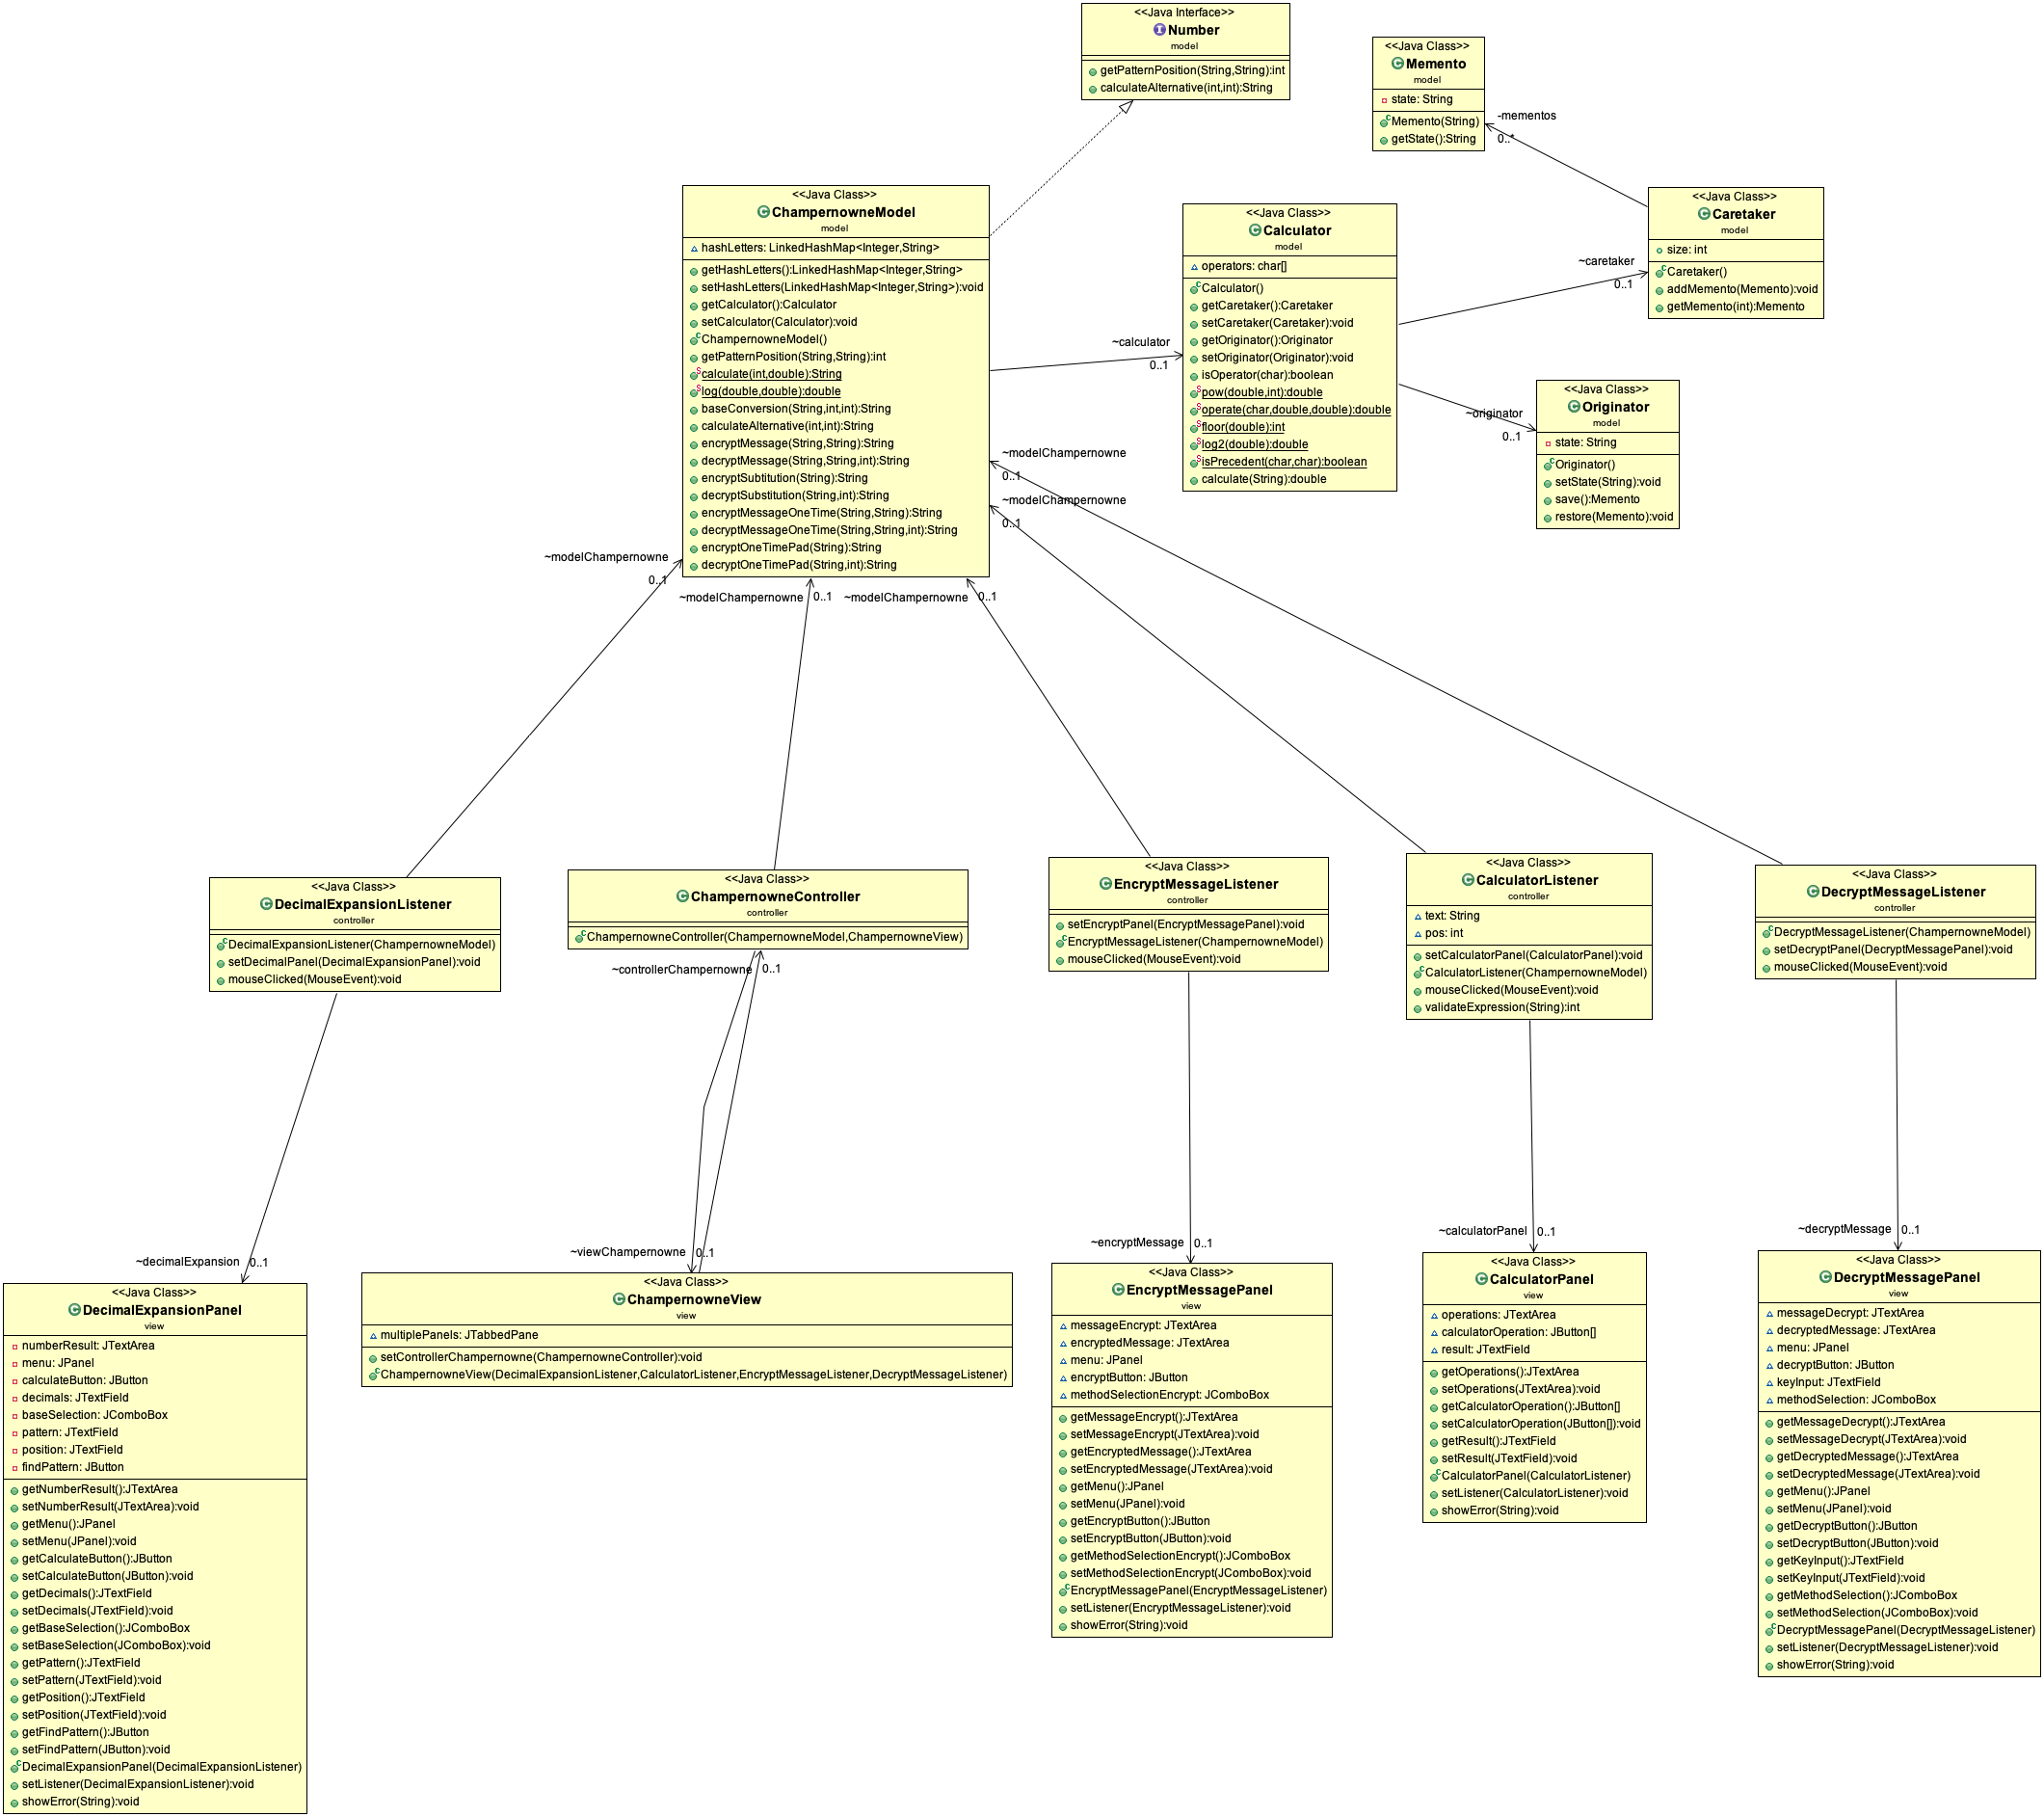
\includegraphics[scale=0.22]{images/ClassDiagramChampernowne.png}
\caption[Class Diagram]{Class Diagram.Personal Creation}
\end{figure}

\begin{figure}[H]
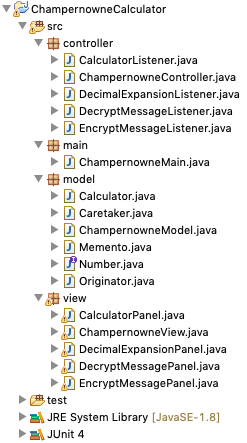
\includegraphics[scale=0.8]{images/directories.png}
\caption[Directory organization]{Directory organization.Personal Creation}
\end{figure}

\subsection{Implementation by View}

The application is form by four panels: Calculator, Champernowne Constant, Encrypt Message and Decrypt Message. This section will describe the user stories implemented in each panel. All the use cases mentioned for the delivery 1 were implemented with their related user story. The use cases related to the basic calculator operation, operation with the number and number applications were covered. \newline

\textbf{Calculator} \\

This view involves the implementation of EN-US-7 related to the execution of basic mathematical operations. The main functions for the implementation of this function are the validateExpression that is in the controller CalculatorListener.java and the calculate function in the model Calculator.java. The view is represented by the CalculatorPanel.java.

The Champernowne Constant is represented by the C10 symbol and the negative sign for number is represented by +/-.

\begin{figure}[H]
\centering
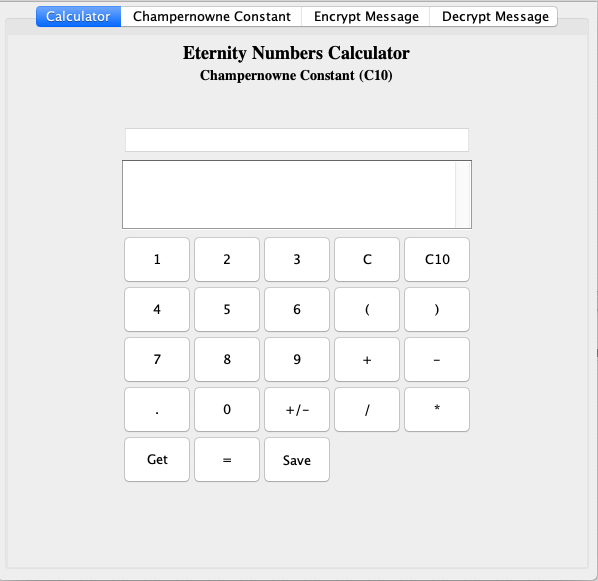
\includegraphics[scale=0.5]{images/CalculatorView.png}
\caption[Calculator View]{Calculator View.Personal Creation}
\end{figure}

\textbf{Champernowne Constant View} \\

This view involves the implementation of EN-US-1 and EN-US-2, since the Champernowne Constant is a built number it was for by the concatenation of strings which provided the possibility of presenting more decimals to the user for the identification of patterns in those decimals. The calculation of the number by formula is also provided for the EN-US-7.

The controller for this view is the DecimalExpansionListener.java, the view the DecimalExpansionPanel.java and the model the ChampernowneModel.java.

\begin{figure}[H]
\centering
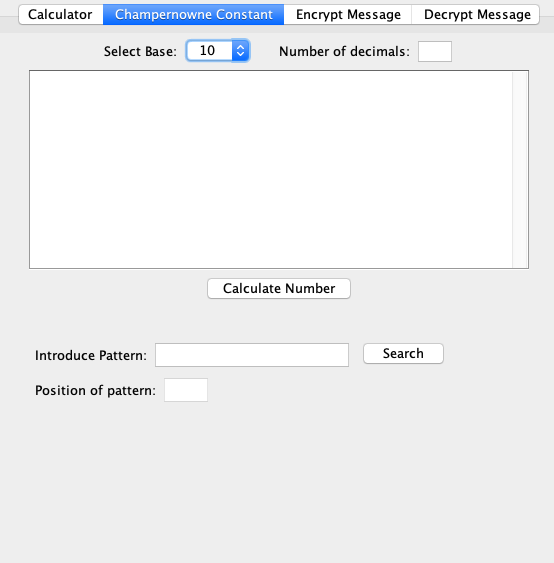
\includegraphics[scale=0.5]{images/DecimalExpansion.png}
\caption[Champernowne Constant View]{Champernowne Constant View.Personal Creation}
\end{figure}

\textbf{Encrypt Message View} \\

This view includes the implementation of the EN-US-3. The substitution cipher was creating by using a hash map with the most common symbols of the language, then selecting a position that represents a starting element in the Champernowne Constant and modifying the letter using the value in that position and the hash getting a new symbol as a result.

The view for this implementation is the EncryptMessagePanel.java, the controller the EncryptMessageListener.java and the model the ChampernowneModel.java.

\begin{figure}[H]
\centering
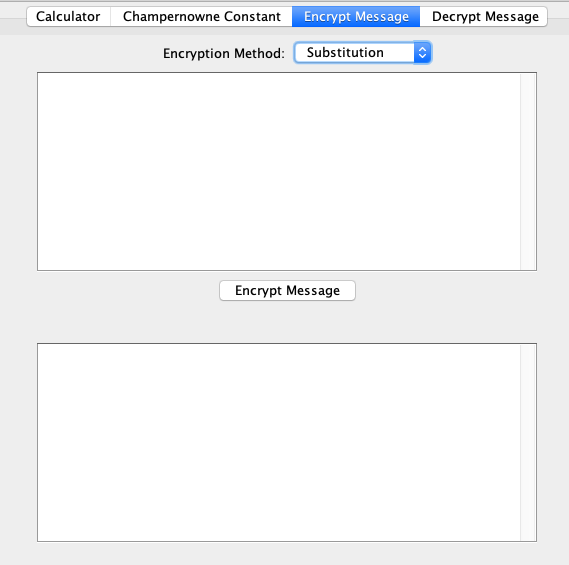
\includegraphics[scale=0.5]{images/EncryptMessage.png}
\caption[Encrypt Message View]{Encrypt Message View.Personal Creation}
\end{figure}

\textbf{Decrypt Message View} \\

This view includes the implementation of EN-US-4. The decryption for the substitution cipher was implementing by reverting the movement previously made according to a position in the Champernowne Constant (the key). 

The view for this implementation is the DecryptMessagePanel.java, the controller the DecryptMessageListener.java and the model the ChampernowneModel.java.

\begin{figure}[H]
\centering
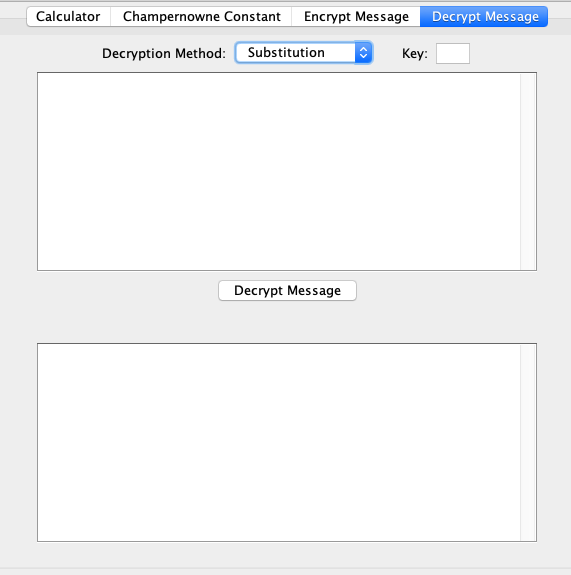
\includegraphics[scale=0.5]{images/DecryptMessage.png}
\caption[Decrypt Message View]{Decrypt Message View.Personal Creation}
\end{figure}

\subsection{Additional Work}

Some unit test case were developed for the most important functions in the model and the controllers using JUnit and the documentation using javadoc. Also, as requested for the interview a prototype of an android application for the calculator was developed. The code is provided in the repository.

\begin{figure}[H]
\centering
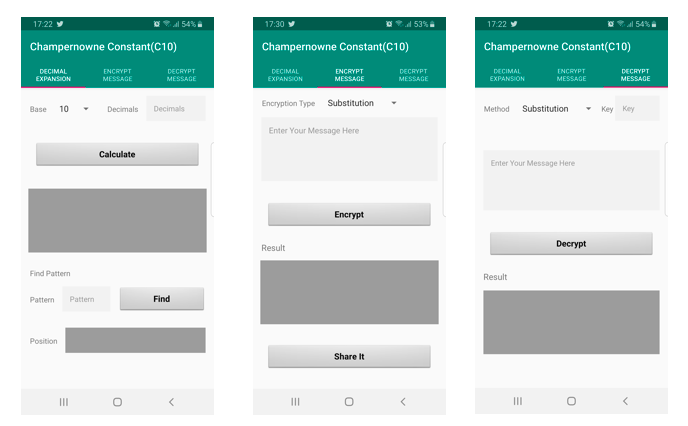
\includegraphics[scale=0.5]{images/Android.png}
\caption[Mobile Application Prototype Views]{Mobile Application Prototype Views.Personal Creation}
\end{figure}
%%%%%%%%%%%%%%%%%%%%%%%%%%%%%%%%%%%%%%%%%%%%%%
\chapter{Conclusion}

The objectives in each problem were achieved, even though the Champernowne Constant is not known for a lot people. The problems allowed to gather different requirements for potential users, gain understanding about the applications and characteristics of the Champernowne Constant, and catch a glimpse of the features that the calculator should have.

It is important to mention that the operation of the calculator are specifically related with the characteristics of the number. The find pattern is possible since the Champernowne Constant is a normal number, and the cryptography features are based on the fact that it is a transcendental number.

This report shows the implementation of the functionalities of the system; it was developed as a first version, multiple modifications can be added in the future. The extensibility features include tackling the global constraints to make a more flexible user interface and provide support for multiple languages.

Additionally, it would be useful to increase the range of action of the encryption and decryption tool by adding other transcendental numbers which would increase the randomness and security of the application. 

\newpage
%%%%%%%%%%%%%%%%%%%%%%%%%%%%%%%%%%%%%%%%%%%%%%%
\newpage
\begin{thebibliography}{9}

\bibitem{website1} 
P. Kantham. USER STORIES IN CONTEXT.(2019). Retrieve from:
\\\texttt{https://users.encs.concordia.ca/~kamthan/courses/soen-6481/user\_stories\_context.pdf}


\bibitem{website2} 
P. Kantham. USER STORIES IN CONTEXT.(2019). Retrieve from:
\\\texttt{https://users.encs.concordia.ca/~kamthan/courses/soen-6481/user\_stories\_context.pdf}

\bibitem{website3}
P. Kantham. TRACEABILITY IN SOFTWARE REQUIREMENTS. (2019). Retrieve from:
\\\texttt{https://users.encs.concordia.ca/\~kamthan/courses/soen-6481/software\_requirements\_traceability.pdf}

\bibitem{website4}
P. Kantham. 1INTRODUCTION TO SOFTWARE PRODUCT QUALITY. (2019). Retrieve from:
\\\texttt{https://users.encs.concordia.ca/\~kamthan/courses/soen-6481/software\_product\_quality\_introduction.pdf}

\bibitem{website5}
M.K. Viswanath. Transcendental Numbers and Cryptography. (2019). Retrieve from:
\\\texttt{http://www.m-hikari.com/ams/ams-2014/ams-173-176-2014/viswanathAMS173-176-2014.pdf}

\bibitem{website6}
J. L. González-Santander. A CIPHER BASED ON THE RANDOM SEQUENCE OF DIGITS IN IRRATIONAL NUMBERS. (2019). Retrieve from:
\\\texttt{http://www.iacis.org/iis/2016/1\_iis\_2016\_14-25.pdf}

\end{thebibliography}

\end{document}
